\section{Задание 2 --- Вычисления в PHP}

Написать программы для решения следующих двух задач:

\begin{enumerate}

\item{Вычисление значения степенного ряда.}

  Дано:

  \begin{itemize}
  \item{натуральное число $n$;}

  \item{действительное число $x$;}
  \end{itemize}
  
  Вычислить значение функции заданной степенным рядом:

  $$f(x) = x - \frac{x^3}{3!} + \frac{x^5}{5!} + ... + (-1)^{n + 1} \frac{x^n}{n!}$$

  Получить результат для $n = 7$ и $x = \pi / 2$.

  Ввод данных:

  \begin{center} 
    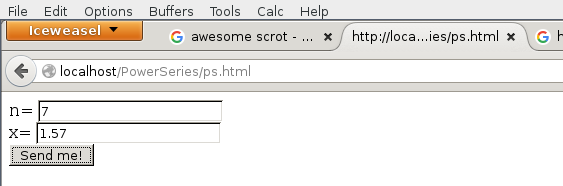
\includegraphics[width=9cm]{img/05.png}
  \end{center}

  Результат:

  \begin{center} 
    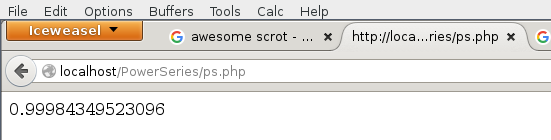
\includegraphics[width=10cm]{img/06.png}
  \end{center}

  Исходный код \verb|ps.html|:

\begin{verbatim}
<form action="ps.php" method="post">
  n=  <input type="text" name="n" /><br />
  x= <input type="text" name="x" /><br />
  <input type="submit" name="submit" value="Send me!" />
</form>
\end{verbatim}

Исходный код \verb|ps.php|:

\begin{verbatim}
<?php
$n = $_POST['n'];
$x = $_POST['x'];
$result = $x;
$fact = 1;
$minusDegree = -1;
for ($i = 3; $i <= $n; $i=$i+2)
{
    if ($i != 1) $fact = $fact * $i * ($i - 1);
    $result = $result + $minusDegree*pow($x, $i)/$fact;
    $minusDegree = $minusDegree * (-1);
}
echo $result;
?>
\end{verbatim}

\item{Обработка данных}

  Дано натуральное число $n$. Переставить его цифры так, чтобы образовалось максимальное число, записанное теми же числами.

  Ввод числа:

  \begin{center} 
    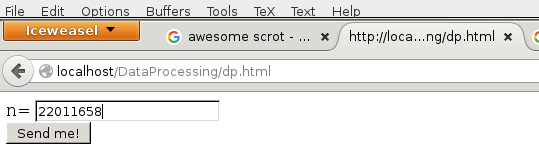
\includegraphics[width=10cm]{img/07.png}
  \end{center}

  Число после перестановок цифр:

    \begin{center} 
    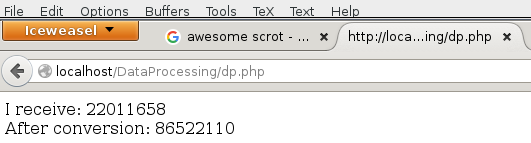
\includegraphics[width=10cm]{img/08.png}
  \end{center}

    Исходный код \verb|dp.html|:
\begin{verbatim}
<form action="dp.php" method="post">
  n=  <input type="text" name="n" /><br />
  <input type="submit" name="submit" value="Send me!" />
</form>
\end{verbatim}

Исходный код \verb|dp.php|:
\begin{verbatim}
<?php
$n = $_POST['n'];
$digitCount = array(0,0,0,0,0,0,0,0,0,0);
$result = 0;
echo "I receive: ";
echo $n;
echo "<br>";
while ($n > 0){
    $digit = $n % 10;
    $digitCount[$digit] = $digitCount[$digit] + 1;
    $n = floor($n / 10);
}
$tens = 1;
for ($i = 0; $i <10; $i = $i + 1){
    for ($j = 1; $j <= $digitCount[$i]; $j = $j + 1){
        $result = $result + $i*$tens;
        $tens = $tens * 10;
    }
}
echo "After conversion: ";
echo $result;
echo "\n";
?>
\end{verbatim}
\end{enumerate}

